%\documentstyle[epsf,twocolumn]{jarticle}       %LaTeX2.09仕様
\documentclass[twocolumn]{jarticle}     %pLaTeX2e仕様
%\documentclass[dvipdfmx,autodetect-engine]{ujarticle}	%???
%%%%%%%%%%%%%%%%%%%%%%%%%%%%%%%%%%%%%%%%%%%%%%%%%%%%%%%%%%%%%%
%%
%%  基本 バージョン
%%
%%%%%%%%%%%%%%%%%%%%%%%%%%%%%%%%%%%%%%%%%%%%%%%%%%%%%%%%%%%%%%%%
\setlength{\topmargin}{-45pt}
%\setlength{\oddsidemargin}{0cm}
\setlength{\oddsidemargin}{-7.5mm}
%\setlength{\evensidemargin}{0cm}
\setlength{\textheight}{24.1cm}
%setlength{\textheight}{25cm}
\setlength{\textwidth}{17.4cm}
%\setlength{\textwidth}{172mm}
\setlength{\columnsep}{11mm}

\kanjiskip=.07zw plus.5pt minus.5pt		%漢字と漢字の間に小さなグルーが入っている?その設定らしい


%【節がかわるごとに(1.1)(1.2) …(2.1)(2.2)と数式番号をつけるとき】tex
%\makeatletter
%\renewcommand{\theequation}{%
%\thesection.\arabic{equation}} %\@addtoreset{equation}{section}
%\makeatother

%\renewcommand{\arraystretch}{0.95} 行間の設定

%%%%%%%%%%%%%%%%%%%%%%%%%%%%%%%%%%%%%%%%%%%%%%%%%%%%%%%%
\usepackage[dvipdfm]{graphicx}   %pLaTeX2e仕様(要\documentstyle ->\documentclass)
%%%%%%%%%%%%%%%%%%%%%%%%%%%%%%%%%%%%%%%%%%%%%%%%%%%%%%%%








\begin{document}

\twocolumn[		%全体を二段表示する場合には,一段表示したい部分を\twocolumn[]で囲めば良い
\noindent
\hspace{1em}

輪講資料  2020年
\hfill
\ \ 多田瑞葵

\vspace{2mm}
\hrule		%これはタイトルを囲む横線
\begin{center}
{\Large \bf 輪講 LaTex 課題}
\end{center}
\hrule
\vspace{3mm}
]

\section{はじめに}
進捗報告や研究発表会の際の資料などに望ましい LaTeX の構成例です.

この PDF の例を見本として, 「practice. tex 」 を元に同じものを作成してください.

名前や日付は適切なものに書き換えてください.

\subsection{課題での留意点}
\begin{itemize}

\item 〜practice〜 の部分を適宜補う
\item 図表を適切な位置に張り付ける
\item 図表に対しては \textbackslash label と \textbackslash ref を使う
\item bibtex を使って参考文献をのせる
\end{itemize}

\section{要素技術}

\subsection{要素技術 1 }
%〜practice〜
要素技術1における式を以下に示す.$x_1, ..., x_n$をデータとすると,出力$y$は
	\begin{equation}
		y = \sum_{i=0}^{n} \frac{\exp{(x_i)}}{x_i}
	\end{equation}
となる.

\subsection{要素技術 2 }
%〜practice〜
%bibtexを引用したいーーー
Bengioらはニューラルネットワーク言語モデルを提案した\cite{FFNN}.Bahdanauらは出力ごとに入力単語に対する荷重を決定してエンコードするアテンションモデルを提案した\cite{translate}.


\section{提案手法}
提案手法はうんたらかんたら〜

\section{実験}
実験をかくかくしかじか〜

	\begin{table}
		\caption{実験結果}
		\begin{tabular}[width=\linewidth]{|c|c|c|c|} \hline
			予測 & 評価回数 & Accuracy[\%] & Baseline[\%] \\ \hline \hline
			投票先 & 160284 & 79.43 & 75.68 \\ \hline
			処刑先 & 21626 & 89.26 & 79.31 \\ \hline
 		\end{tabular}
		\label{tb:data}
	\end{table}

	\begin{figure}
		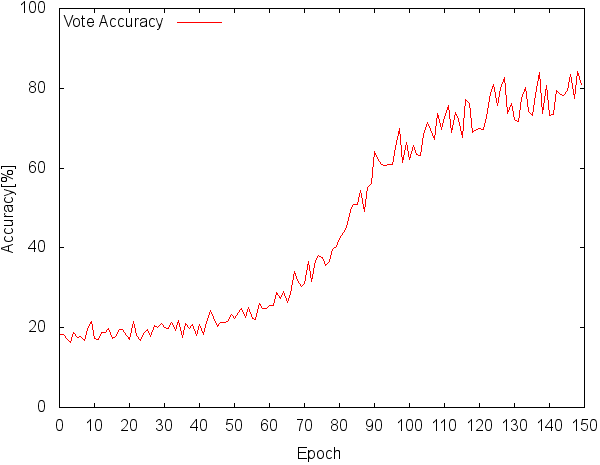
\includegraphics[width=\linewidth]{accuracy.png}		%文書の幅に合わせて図を貼る
		\caption{Accuracy の推移}
		\label{fig:accuracy}
	\end{figure}


\section{実験結果}
%〜practice〜
表\ref{tb:data}に実験結果を示す.図\ref{fig:accuracy}にAccuracyの推移を示す.

\section{今後の課題}
今後の課題はうんぬんかんぬん〜


\bibliography{index}		%文献データベースindex.bibを使用する
\bibliographystyle{unsrt} 	%参考文献出力スタイル
% junsrtにするとエラーが出る,なぜ?

%メモ
%journalの項目が必要なのはarticle

\end{document}
